\documentclass{article}

\usepackage[margin=1in]{geometry}
\usepackage{amsmath}
\usepackage{amsfonts}
\usepackage{graphicx}


\title{Homework 7: Advanced Linear Systems (ECEN 5448)}
\author{Zachary Vogel}
\date{\today}


\begin{document}
\maketitle

\section*{Problem 1}
The problem asks us to consider to matrices and answer a few questions about them. The Matrices are:
\[A=\begin{pmatrix}1 & 3\\0 & 1\end{pmatrix}\]
\[B=\begin{pmatrix}2 & -4\\1 & 4\end{pmatrix}\]
\subsection*{(a)}
The first question asks which of the matrices are positive definite. Take any non-zero vector $x=\begin{pmatrix}a & b\end{pmatrix}^T$. Multiply $x^T$ and x.
\[x^TAx=\begin{pmatrix}a &b\end{pmatrix}\begin{pmatrix}a+3b\\b\end{pmatrix}=a^2+3ab+b^2\]
So, if $a^2+b^2>-3ab$ for all a and b this matrix is positive definite. This isn't true because of the simple counter example $a=1$ and $b=-1$.
Now, let us examine the other matrix. We take a different approach here, finding the Hermitian part of the matrix.
\[A_H=\frac{1}{2}\left(A+A^H\right )=\begin{pmatrix}1 & -2\\\frac{1}{2} & 2\end{pmatrix}+\begin{pmatrix}1 & \frac{1}{2}\\-2 &2\end{pmatrix}=\begin{pmatrix}2 &-1.5\\-1.5&4\end{pmatrix}\]
Now, we can check the positive definiteness of this very easily by finding its eigenvalues. The eigenvalues are positive so this second matrix must be positive definite.

\subsection*{(b)}
Now the problem wants to know two norms, first the induced matrix norm defined by the 2 norm. Then the induced norm defined by the infinity norm.\\
First, for the matrix A. The infinity norm will be the maximum row sum of the matrix.
\[\lvert\lvert A\rvert\rvert_{\infty}=\max_{i\leq 1\leq m}\sum_{j=1}^n\lvert a_{ij}\rvert=1+3=4\]
The 2 norm of the matrix a is defined as:
\[\lvert\lvert A\rvert\rvert_2=\sqrt{\lambda_{\text{max}}(A^HA)}\]
\[\sqrt{\lambda_{\text{max}}(A^HA)}=\sqrt{\lambda_{\text{max}}\begin{pmatrix}5&-4\\-4&32\end{pmatrix}}=\sqrt{32.5801}=5.7079\]
Doing the same thing for the matrix B.
\[\lvert\lvert B\rvert\rvert_{\infty}=6\]
\[\sqrt{\lambda_{\text{max}}(A^HA)}=\sqrt{1}=1=\lvert\lvert B\rvert\rvert_2\]

\subsection*{(c)}
The final part of this problem asks us to use MATLAB to draw the image of the unit circle for each one of the above A matrices. This is defined by $\{Ax\big|x\in\mathbb{R}^2,\lvert\lvert x\rvert\rvert=1\}$. Then it wants to know what the two matrix norms from part b represent in these plots.\\
The plots of these figures are below:
\begin{figure}[h!]
    \centering
    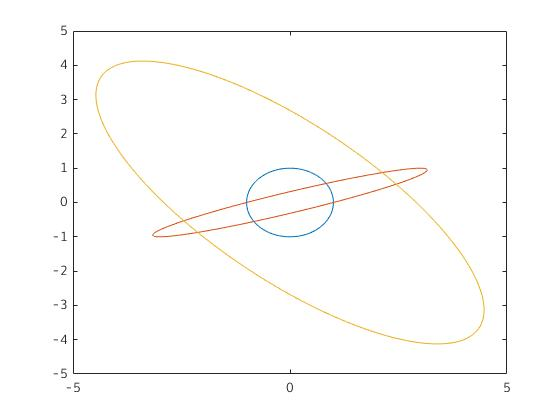
\includegraphics[width=0.5\textwidth]{2norm.jpg}
\end{figure}
\begin{figure}[h!]
    \centering
    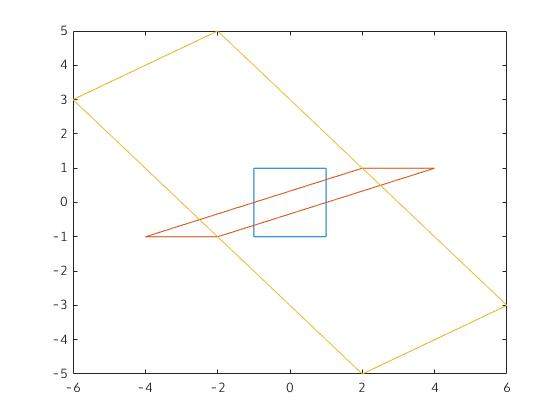
\includegraphics[width=0.5\textwidth]{infnorm.jpg}
\end{figure}
The first image is for the $L_2$ norm, and the second is for the $L_\infty$ norm. In the first image, the ellipses are the $L_2$ norms for all xs on the circle times the matrices. Similarly, in the second image, the parallelograms are the infinity norm of the matrices times various xs. The induced norms from part b represent the maximum distance from the center of the circle/square to the edge of these images.
\section*{Problem 2}
Here, consider the matrix:
\[A=\begin{pmatrix}-1 & -1\\2 & -3\end{pmatrix}\]
The problem wants a proof that this is a Hurwitz matrix. Given that that is true, it wants a quadratic Lyapunov function for the dynamics $\dot{x}=Ax$.\\
To show this is a Hurwitz matrix, we find the eigenvalues with the characteristic equation.
\[c(\lambda)=(-1-\lambda)(-3-\lambda)+2=\lambda^2+4\lambda+5\]
\[\lambda=-2\pm j\]
Thus, this is a Hurwitz matrix because it has negative eigenvalues. Due to the theorem proven in class, we know that for $Q=I$ we can find a P such that:
\[PA+A^TP=-Q\]
This is a linear system and can thus be solved by multiplying out:
\[\begin{pmatrix}a &b\\b&c\end{pmatrix}\begin{pmatrix}-1 &-1\\2 &-3\end{pmatrix}+\begin{pmatrix}-1 & 2\\-1&-3\end{pmatrix}\begin{pmatrix}a &b\\b&c\end{pmatrix}=\begin{pmatrix}-1 & 0\\0&-1\end{pmatrix}\]
This yields the following:
\[-2a+4b=-1\]
\[2c-a-4b=0\]
\[-a-4b+2c=0\]
\[-2b-6c=-1\]
Two of these are the same as one would expect. Now make a matrix to solve:
\[\begin{pmatrix}-2 &4 &0\\-1& -4&2\\0 &-2&-6\end{pmatrix}\begin{pmatrix}a\\b\\c\end{pmatrix}=\begin{pmatrix}-1\\0\\-1\end{pmatrix}\]
Solving with Matlab gives, $a=-0.45,b=0.025,c=-0.175$. Thus, P is:
\[P=\begin{pmatrix}-0.45 & 0.025\\0.025 & -0.175\end{pmatrix}\]
The Lyapunov function is:
\[V(x)=x^TPx=\begin{pmatrix}x_1&x_2\end{pmatrix}\begin{pmatrix}-0.45x_1+0.025x_2\\0.025x_1-0.175x_2\end{pmatrix}=-0.45x_1^2+0.05x_1x_2-0.175x_2^2\]

\section*{Problem 3}
Here we will once again consider the inverted pendulum:
\[\dot{x}=\begin{pmatrix} x_2\\\sin(x_1)-\mu x_2\end{pmatrix}+\begin{pmatrix}0\\ u(t)\end{pmatrix}\]
where $\mu>0$ is a friction constant. Then it wants us to show that the equilibrium at $x=\begin{pmatrix}\pi &0\end{pmatrix}^T$ is locally exponentially stable for the original (unforced) nonlinear system.\\
Since the system is unforced, it can be written as:
\[\dot{x}=Ax+f(x,t)=\begin{bmatrix}0&1\\-1&-\mu\end{bmatrix}\begin{bmatrix}x_1-\pi\\x_2\end{bmatrix}+\begin{bmatrix}0\\x_1-\pi+\sin(x_1)\end{bmatrix}\]
where:
\[\lvert\lvert f(x,t)\rvert\rvert\leq \delta\lvert\lvert x\rvert\rvert^2\]
near the equilibrium of $x=\begin{bmatrix}\pi\\0\end{bmatrix}$. This can be seen more clearly by considering the taylor series expansion of $\sin(x)$ about $\pi$:
\[\sin(x)\approx (x-\pi)-\cfrac{(x-\pi)^3}{3!}+\cfrac{(x-\pi)^5}{5!}-\dots\]
Note that the first term of the series cancels the other terms in $f(x,t)$. Then, we have a leading term $\frac{(x-\pi)^3}{3!}$ which is smaller than $x^2$ for $x$ close to $\pi$. Using this, we can say that if the linearization is Hurwitz, the system is locally exponentially stable by the application proven in class. Since, $0*-\mu-(-1)*1=1>0$ this matrix is Hurwitz, and the system is locally exponentially stable near the equilibrium point here.\\

\section*{Problem 4}
Consider the previous problem, where $(0,0)$ is not a stable equilibrium. Linearize the system about the point $(0,0)$. At that point, $u(t)$ can be considered as the torque that is applied to the pendulum. Now, consider the feedback P-control law: $u(t)=-\alpha x_1$ for the linearized system. Now answer these two things.\\
The linearized system is:
\[\dot{x}=Ax+Bu=\begin{bmatrix}0 & 1\\1 & -\mu\end{bmatrix}\begin{bmatrix}x_1\\x_2\end{bmatrix}+\begin{bmatrix}0\\1\end{bmatrix}u(t)\]
\subsection*{(a)}
Show that for some gain $\alpha>0$, the origin is exponentially stable for the closed-loop system (i.e. when we let $u(t)=-\alpha x_1$).\\
Here, we write the system:
\[\dot{x}=Ax+f(x,t)=\begin{bmatrix}0 & 1\\1-\alpha &-\mu\end{bmatrix}\begin{bmatrix}x_1\\x_2\end{bmatrix}+\begin{bmatrix}0\\-x_1+\sin(x_1)\end{bmatrix}\]
We know from the previous problem that this system is stable if $1-\alpha<0$, so as long as $\alpha>1$ this system is stable.\\
\subsection*{(b)}
Suppose that $u(t)=-\alpha x_1+d(t)$ where $d(t)$ is a disturbance in the input of the system. Let output $y(t)=x_1(t)$ be the position of the pendulum. Find the $\mathfrak{L}_{\infty}$ gain of the system from this disturbance to the output.\\
Didn't have time, will start earlier now that we are getting into topics I'm not as proficient at.

\section*{Problem 5}
This problem wants a proof that $\lvert\lvert A\rvert\rvert_{\text{ind.},2}=\lambda_{\text{max}}(A)$ for a positive definite matrix A. This fact was used several times in the proof of Lyapunov theorems.\\
Since A is positive definite, we know a few things about it. First, its determinant is greater than 0. This implies it has full rank, and can be diagnolized. Now, we remember the definition of the matrix norm:
\[\lvert\lvert A\rvert\rvert=\sup_{x\neq 0}\frac{\lvert\lvert Ax\rvert\rvert_2}{\lvert\lvert x\rvert\rvert_2}\]
Now, assume that $e_i$ is an eigenvector of $A$. Then we can write:
\[\lvert\lvert Ae_i\rvert\rvert=\lvert\lvert \lambda_ie_i\rvert\rvert=\lvert\lambda_i\rvert\lvert\lvert e_i\rvert\rvert\]
and by Cuachy Schwarz inequality we can say:
\[\lvert\lvert Ae_i\rvert\rvert\leq \lvert\lvert A\rvert\rvert\lvert\lvert e_i\rvert\rvert\]
and we make an inequality:
\[\lvert \lambda_i\rvert\lvert\lvert e_i\rvert\rvert\leq \lvert\lvert A\rvert\rvert\lvert\lvert e_i\rvert\rvert\]
And thus that:
\[\lvert \lambda_i\rvert\leq \lvert\lvert A\rvert\rvert\]
Now we just need to show that:
\[\lvert \lambda_i\rvert_2\geq \lvert\lvert A\rvert\rvert_2\]
First note that there exists an orthonormal eigenvector $e_i$ such that $Ae_i=\lambda_ie_i$. Then we can write $x=\sum_i x_ie_i$. Thus:
\[Ax=\sum_ix_i\lambda_ie_i\]
Then, one can write out the norm:
\[\lvert\lvert Ax\rvert\rvert_2^2=\sum_i\lambda_i^2x_i^2\]
Then, you can bound the left side:
\[\lvert\lvert Ax\rvert\rvert_2^2\leq \max{\lvert\lambda_i\rvert}\sum_ix_i^2\]
Taking the square root and dividing by $\lvert\lvert x\rvert\rvert_2$ gives:
\[\cfrac{\lvert\lvert Ax\rvert\rvert}{\lvert\lvert x\rvert\rvert}\leq \lvert \max{\lvert lambda_i\rvert}\]
The left side is the induced 2 norm of A and as we can see it must be less than or equal to the maximum eigenvalue of A. From both of the two previous results, we can see that:
\[\lvert\lvert A\rvert\rvert_2=\lambda_{\text{max}}(A)\]

\end{document}
